\documentclass[]{article}

\usepackage{hyperref}
\usepackage[parfill]{parskip}
\usepackage{titling}
\usepackage[a4paper, margin=1in]{geometry}
\usepackage{graphicx}
\usepackage[T1]{fontenc}
\usepackage{amssymb}
\usepackage{tabu}
\usepackage{float}
\usepackage{wrapfig}
\usepackage[svgnames]{xcolor}

\pretitle{%
	\begin{center}
		\LARGE
		
\includegraphics[width=6cm]{CSS-block}\\[\bigskipamount]
}
\posttitle{\end{center}}

\renewcommand{\familydefault}{\sfdefault}

%opening
\title{University of Bristol Computer Science Society \\ Sponsorship Packages 2016-17}
\author{}
\date{}

\begin{document}

\maketitle

Welcome!

We are the University of Bristol Computer Science Society (CSS). We represent the interests of all Computer Science students at the University. 

We work to support students and staff within our Computer Science community---we organise social events; connect students with opportunities in industry and tackle any issues faced by our members.

We serve a large pool of students, with a diverse range of interests and future career paths, and we'd love to connect you with them!

\section*{Why sponsor us?}

\begin{itemize}
	\item Our department is consistently considered to be \textbf{in the top five Computer Science departments} in the UK.
	\item We do not charge students for membership. \textbf{Anyone studying Computer Science at the University of Bristol is automatically a member of CSS.} We have over 500 undergraduates, as well as more than 200 postgraduates, making us one of the largest societies at the University.
	\item \textbf{We run a number of popular events each year}: hackathons, discussion panels, talks, social events and more. These are a perfect opportunity for you to get involved and promote your brand to our students. We are also keen to help you stage your own event---whether it be a large interactive event or a lunchtime tech talk.
	\item We \textbf{work with other societies} in the University, including:
			\begin{itemize}
				\item The University of Bristol Engineering Society (TUBES)
				\item Bristol Electrical and Electronic Engineering Society (BEEES)
				\item Women In Engineering
				\item LGBT+ Engineers
			\end{itemize}
	\item We are in \textbf{constant communication with our members}, through our:
			\begin{itemize}
				\item Facebook group (1300+ members including many alumni)
				\item Website \footnote{\url{http://cssbristol.co.uk/}} (recently relaunched)
				\item Twitter account (220 followers) \footnote{\url{https://twitter.com/cssbristol}}
				\item Regular email newsletter (commencing September)
                \item Physical noticeboard in the department (commencing September)
			\end{itemize}
		 We can help you promote your message through all of these channels, as well as branding our major events and society t-shirts.
\end{itemize}


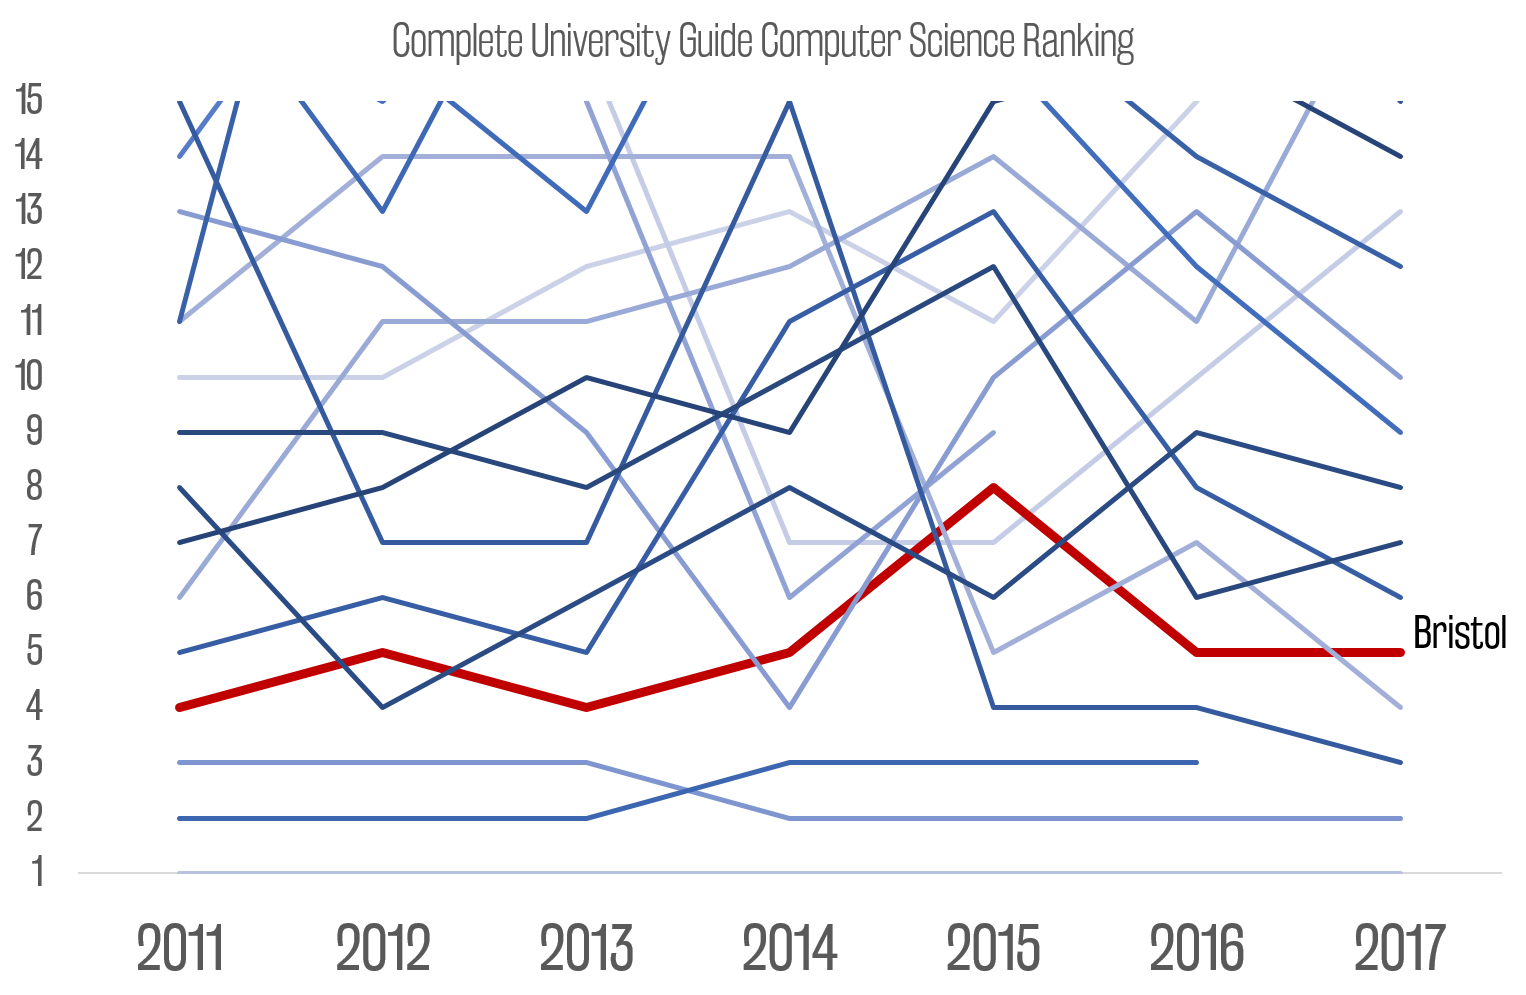
\includegraphics[width=0.5\textwidth]{ranking-chart}  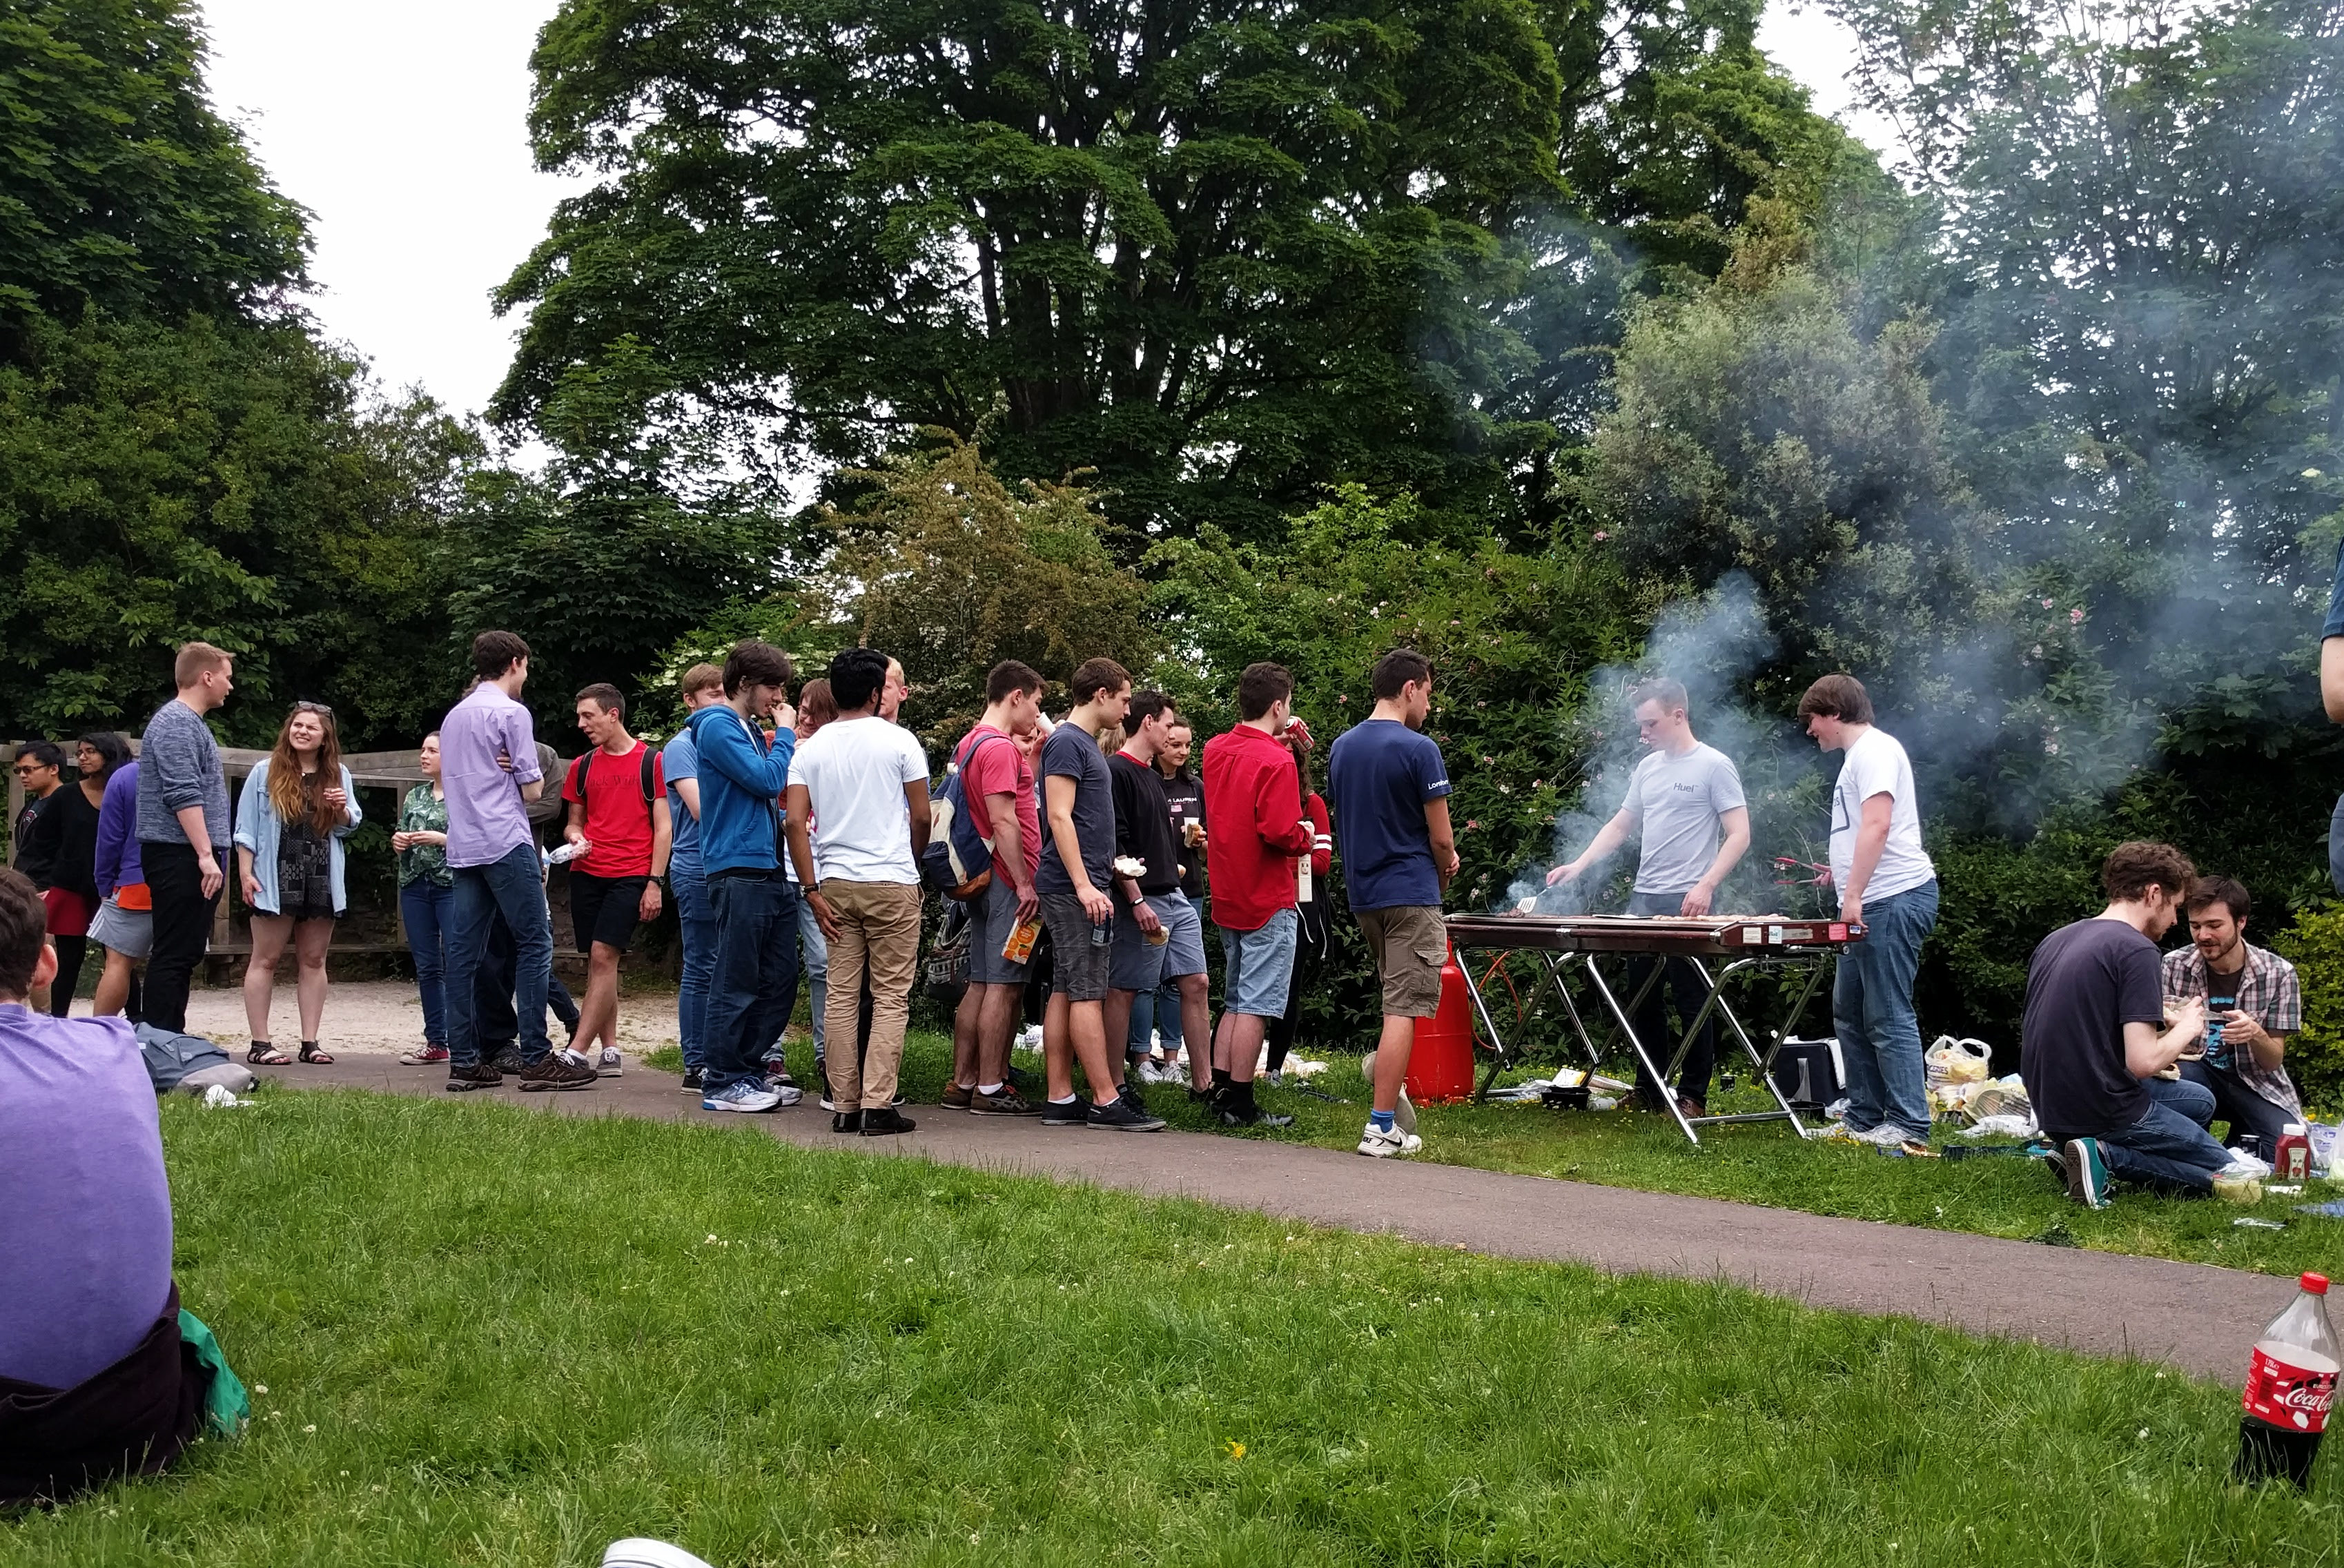
\includegraphics[width=0.5\textwidth]{bbq}

\section*{What options are available?}

We have a number of sponsorship options available. 

\subsection*{Sponsor us for a year}

We recommend investing in a year-long sponsorship of CSS. We have several suggested sponsorship tiers, but don't hesitate to ask us if you're looking for something specific!

\subsubsection*{Bronze {\color{Sienna}(\pounds 899 inc. VAT)}}

\begin{itemize}
	\item Your \textbf{logo appears on our website}
	\item \textbf{Promote job opportunities}/internships/events through our regular email newsletter and website
	\item \textbf{Put up posters} in the Faculty of Engineering \textbf{twice} during your sponsorship
    \item You will be prioritised over non-sponsors if yo
\end{itemize}

\subsubsection*{Silver {\color{Gray}(\pounds 1199 inc. VAT)}}

\begin{itemize}
	\item \emph{Everything in the Bronze package}, plus:
	\item Your \textbf{logo appears on society hoodies}, t-shirts and other merchandise we release during your sponsorship
	\item You will be \textbf{invited to the Computer Science Society Careers day}
	\item Priority timeslot for one \textbf{catered lunch or dinner talk} (in addition to the self-catered talk)
	\item Priority placement on our email newsletter, Facebook group and website
	\item Put up posters in the Faculty of Engineering a total of \textbf{four times} during your sponsorship
\end{itemize}

\subsubsection*{Gold {\color{Goldenrod}(\pounds 1499 inc. VAT)}}

\begin{itemize}
	\item \emph{Everything in the Bronze and Silver packages}, plus:
	\item \textbf{Priority placement} at the Computer Science Society Careers day
	\item Get involved with our \textbf{annual hackathon} or another one of our popular events. Alternatively, host your own event
	\item Up to once per month, communicate your job opportunities/internships/events in \textbf{dedicated emails} to our members
	\item Put up posters in the Faculty of Engineering up to \textbf{once per month} during your sponsorship
\end{itemize}

\subsubsection*{Summary}

\def\arraystretch{1.5}

\begin{tabu} to \textwidth { |X[3,l]|X[c]|X[c]|X[c]| }
	\hline
    										& Bronze & Silver & Gold \\
    \hline
    \multicolumn{4}{|l|}{\textbf{Logo on our}} \\
    \hline
    Website									& \checkmark & \checkmark & \checkmark \\
    Society hoodies 						& 			 & \checkmark & \checkmark \\
    Society t-shirts						&            & \checkmark & \checkmark \\
    \hline
    \multicolumn{4}{|l|}{\textbf{Project fair}} \\
    \hline
    Invitation          					&            & \checkmark & \checkmark \\
    Your own stand		  					&            &            & \checkmark \\
    \hline
    \multicolumn{4}{|l|}{\textbf{Major events (Hackathon, barbecue etc.)}} \\
    \hline
    Brand an event        					&            &            & \checkmark \\
    Or host your own event  				&            &            & \checkmark \\
    \hline
    \multicolumn{4}{|l|}{\textbf{Lunch/dinner talks}} \\
    \hline
    Catered talk							&            & 1		  & 1 \\
    \hline
    \multicolumn{4}{|l|}{\textbf{Communicate with our members}} \\
    \hline
    Profile on our website             		& \checkmark & \checkmark & \checkmark \\
    Your website postings prioritised 		& \checkmark & \checkmark & \checkmark \\
    Advertise in our email newsletter		&            & \checkmark & \checkmark \\
    Post on the society notice board        &            & \checkmark & \checkmark \\
    Dedicated email to all society members  &            &            & \checkmark \\
    \hline
    \multicolumn{4}{|l|}{\textbf{Advertise in the faculty}} \\
    \hline
    Put up posters                          & Twice      & Four times & Monthly \\
    \hline
\end{tabu}

\subsection*{Sponsor a single event}

We highly recommend sponsoring us for the whole year, as this allows us to prioritise you over the many requests we receive to advertise opportunities and talks. We won't always be able to accommodate these requests---but we can guarantee such opportunities to our main sponsors.

\subsubsection*{Event (\textasciitilde\pounds 300--800 ex. VAT)}

CSS holds many events during the year. This year is no different! We have lots planned, including industry-supported activities, CS discussion panels, our annual hackathon, our summer barbecue and much more. Please get in touch to discuss the event you'd like to sponsor. Have your own idea for an event? Let us know and we'll see what we can do!

In return, you will have the opportunity to:

\begin{itemize}
	\item Name the event
	\item Include your name/logo in any event advertising
	\item Send representatives to the event
	\item Give a short (\textasciitilde 10 minutes) presentation to attendees
	\item Place your name/logo on our website
\end{itemize}

\subsubsection*{Tech talk (\pounds 250 ex. VAT)}

Throughout the year, we invite engineers---often CSS alumni---to talk about their experiences in industry and their technical work. You send the presenter, we provide food, drink, venue and faculty-wide advertising.

We usually expect a mixed audience of around 40--50 people, though this varies depending on the availability and interest of students. We can provide advice to help you make your talk attractive to our members.

\section*{How do I sponsor you?}

We'd love to hear from you.

The best way to get in touch is to email our society vice-president, Codrin Popa (vice-president@cssbristol.co.uk). Alternatively, you can email our society president, Hakeem Kushoro (president@cssbristol.co.uk). Let us know which packages you are interested in, and any questions you might have.

\end{document}
